%%%%%%%%%%%%%%%%%%%%%%%%%%%%%%%%%%%%%%%%%%%%%%%%%%%%%%%%%%%%%%%%%%
%%%%%%%% ICML 2015 EXAMPLE LATEX SUBMISSION FILE %%%%%%%%%%%%%%%%%
%%%%%%%%%%%%%%%%%%%%%%%%%%%%%%%%%%%%%%%%%%%%%%%%%%%%%%%%%%%%%%%%%%

% Use the following line _only_ if you're still using LaTeX 2.09.
%\documentstyle[icml2015,epsf,natbib]{article}
% If you rely on Latex2e packages, like most moden people use this:
\documentclass{article}

% use Times
\usepackage{times}
% For figures
\usepackage{graphicx} % more modern

\graphicspath{ {figures/} }
%\usepackage{epsfig} % less modern
\usepackage{subfigure} 

% For citations
\usepackage{natbib}

% For algorithms
\usepackage{algorithm}
\usepackage{algorithmic}

% As of 2011, we use the hyperref package to produce hyperlinks in the
% resulting PDF.  If this breaks your system, please commend out the
% following usepackage line and replace \usepackage{icml2015} with
% \usepackage[nohyperref]{icml2015} above.
\usepackage{hyperref}

% Packages hyperref and algorithmic misbehave sometimes.  We can fix
% this with the following command.
\newcommand{\theHalgorithm}{\arabic{algorithm}}

% Employ the following version of the ``usepackage'' statement for
% submitting the draft version of the paper for review.  This will set
% the note in the first column to ``Under review.  Do not distribute.''
%\usepackage{icml2015} 

% Employ this version of the ``usepackage'' statement after the paper has
% been accepted, when creating the final version.  This will set the
% note in the first column to ``Proceedings of the...''
\usepackage[accepted]{icml2015}
\usepackage{amssymb}
\usepackage{amsmath}


% The \icmltitle you define below is probably too long as a header.
% Therefore, a short form for the running title is supplied here:
%\icmltitlerunning{Submission and Formatting Instructions for ICML 2015}

\begin{document} 

\twocolumn[
\icmltitle{Exploring the Naturalness of Buggy Code with Recurrent Neural Networks}

% It is OKAY to include author information, even for blind
% submissions: the style file will automatically remove it for you
% unless you've provided the [accepted] option to the icml2015
% package.
\icmlauthor{Jack Lanchantin}{jjl5sw@virginia.edu}
\icmladdress{University of Virginia, Department of Computer Science}
\icmlauthor{Ji Gao}{email@coauthordomain.edu}
\icmladdress{University of Virginia, Department of Computer Science}

% You may provide any keywords that you 
% find helpful for describing your paper; these are used to populate 
% the "keywords" metadata in the PDF but will not be shown in the document
%\icmlkeywords{boring formatting information, machine learning, ICML}

\vskip 0.3in
]

\begin{abstract} 
Statistical language models are powerful tools which have been used for many tasks within natural language processing.
Recently, they have been used for other sequential data such as source code. \cite{ray2015naturalness} 
\end{abstract} 

\section{Introduction}
\label{introduction}
Natural language is inherently very well understood by humans. There are certain linguistics and structures associated with natural language which make it fluid and efficient. These repetitive and predictive properties of natural language make it easy to exploit via statistical language models. Although the actual semantics are very much different, source code is also repetitive and predictive. Some of this is constrained by what the compiler expects, and some of it is due to the way that humans construct the code. Regardless of why it is predictable, it has been shown that code is accommodating to the same kinds of language modeling as natural language  \citep{hindle2012naturalness}. 

The language modeling task is defined as estimating the probability of a sequence of words (or tokens). Formally,
given a sequence of tokens S a language model attempts to estimate the probability of S occurring in the language via the following equation:

\begin{align*}
P(S) = P(s_{1}) \prod_{i=2}^{N} P(s_t \vert s_1,s_2, ... , s_{t-1})
\end{align*}


Where the conditional probabilities $P(s_t \vert s_1,s_2, ... , s_{t-1})$ model the probability of token $s_t$ occurring given all previous tokens $s_1,s_2, ... , s_{t-1}$.

From a distribution such as a language model, we can measure the entropy, or amount of uncertainty of a given sequence $S$. Using this metric, we can determine particular sequences which are ``unnatural'' with respect to the language. 

Recently, \cite{ray2015naturalness} showed that it is possible to predict buggy lines of code based on the entropy of the line with respect to a code language model.  In this work, the authors proposed a $cache language model$, which is an extension of an $n-gram$ language model to handle local regularities in a piece of code which is being examined for bugs. They provide extensive experimentation to show that entropy of code can successfully be used to determine buggy lines similar to, and in some cases better than previous state-of-the-art bug localization tasks.

The main drawback of their paper is that they use a typical $n-gram$ language model, which struggles to handle long term dependencies due to the computation cost of a large $n$. There has been much recent work which has shown that recurrent neural network models are able to model languages with long term dependencies much better than previous techniques \cite{graves2013generating, sutskever2014sequence, sundermeyer2012lstm, karpathy2015visualizing}. 





%The problem is that the conditional probabilities become intractable when the sequences are very long. In order to handle this, researchers typically use $n$-$gram$ models, which alleviate modeling all previous tokens by only using $n$ previous tokens. Thus, $n$-$gram$ conditional probabilities are modeled as: 

\begin{align*}
P_{ngram}(s_t \vert s_1,s_2, ... , s_{t-1}) = P(s_t \vert s_{t-n+1},...,s_{t-1})
\end{align*}





\section{Related Work}

\subsection{Bug Dection}
For software bug detection, there are two main areas of research: bug prediction, and bug localization. \\
Bug prediction, or statistical defect prediction, which is concerned with being able to predict whether or not there is a bug in a certain piece of code, has been widely studied in recent years \citep{catal2009systematic}. With the vast amount of archived repositories in websites such as github.com, there are many opportunities for finding bugs in code.\\
Static bug finders (SBFs), automatically find where in code a bug is located. SBFs use properties of code to indicate locations of bugs. There has been a wide array of recent work in this area \citep{rahman2014comparing}, which use many pattern recognition techniques to find bugs. As noted in \cite{ray2015naturalness}, using SBFs and using the entropy of language models are two very different approaches to achieve the same goal. The main goal of their work is to compare the effectiveness of language models vs SBFs for the same task of classifying buggy lines.

\subsection{Natural Language Processing}
There have been many works in NLP which use language models for sequence to sequence tasks, such as word completion, machine translation, and many others. There are also a variety of models which use word embeddings trained on language models in order to perform other tasks such as sequence classification (e.g. sentiment analysis). 

Separately, there are a variety of models which do not use language models, but do sequence classifications using pattern recognition techniques. These would be similar to SBF techniques in software engineering. However, to the best of our knowledge, there have not been any works in NLP which use entropy from neural language models to classify sequences.

\section{Methods}

\subsection{Recurrent Neural Network Language Model}

Recurrent neural networks (RNNs) are models which are particularly well suited for modeling sequential data.
At each time step $t$, an RNN takes an input vector $\mathbf{x_t} \in \mathbb{R}$ and a hidden state vector $\mathbf{h_{t-1}} \in \mathbb{R}^m$ and produces the next hidden state $\mathbf{h_{t}}$ by applying the following recursive operation:

\begin{equation}
\mathbf{h_{t}} = f(\mathbf{Wx_{t }}+ \mathbf{Uh_{t-1}} + \mathbf{b})
\end{equation}

Where $\mathbf{W} \in \mathbb{R}^{m \times n}, \mathbf{U} \in \mathbb{R}^{m \times m}, \mathbf{b} \in \mathbb{R}^{m}$ are the learnable parameters of the model, and $f$ is an element-wise nonlinearity. The parameters of the model are learnt via backpropagation through time. Due to their recursive nature, RNNs can model the full conditional distribution of any sequential distribution. However, RNNs suffer from what is referred to as the ''vanishing gradient'' problem, where the gradients of time steps far away either vanish toward 0, or explode toward infinity, thus making the optimization of the parameters difficult.

To handle the exploding gradients problem, \cite{hochreiter1997long} proposed Long Short-term Memory (LSTM), which can handle long term dependencies by using ``gating'' functions which can control when information is written to, read from, and forgotten. Specifically, LSTM ``cells'' take inputs $\mathbf{x_t}, \mathbf{h_{t-1}} $, and $\mathbf{c_{t-1}} $, and produce $\mathbf{h_{t}}$ , and $\mathbf{c_{t}} $ in the following way:

\begin{align*}
\bf{i_t} &= \sigma(\bf{W^ix_t} + U^ih_{t-1} + b^i) \\
\bf{f_t} &= \sigma(\bf{W^fx_t} + U^fh_{t-1} + b^f) \\
\bf{o_t} &= \sigma(\bf{W^ox_t} + U^oh_{t-1} + b^o) \\
\bf{g_t} &= tanh(\bf{W^gx_t} + U^gh_{t-1} + b^g) \\
\bf{c_t} &= f_t \odot c_{t-1} + i_t \odot g_t \\
\bf{h_t} &= o_t \odot tanh(c_t)
\end{align*}

Where $\sigma()$ and $tanh()$ are element-wise sigmoid and hyperbolic tangent functions. $\odot$ represents and element-wise multiplication. $\bf{i_t}$, $\bf{f_t}$, and $\bf{o_t}$ are referred to as the input, forget, and output gates, respectively. An overview of an LSTM module can be seen in Figure \ref{fig:LSTM} It is the gating mechanisms that allow the LSTM to remember long term dependencies, which are especially important in code where a certain line may depend on code many lines back. 


\begin{figure}
  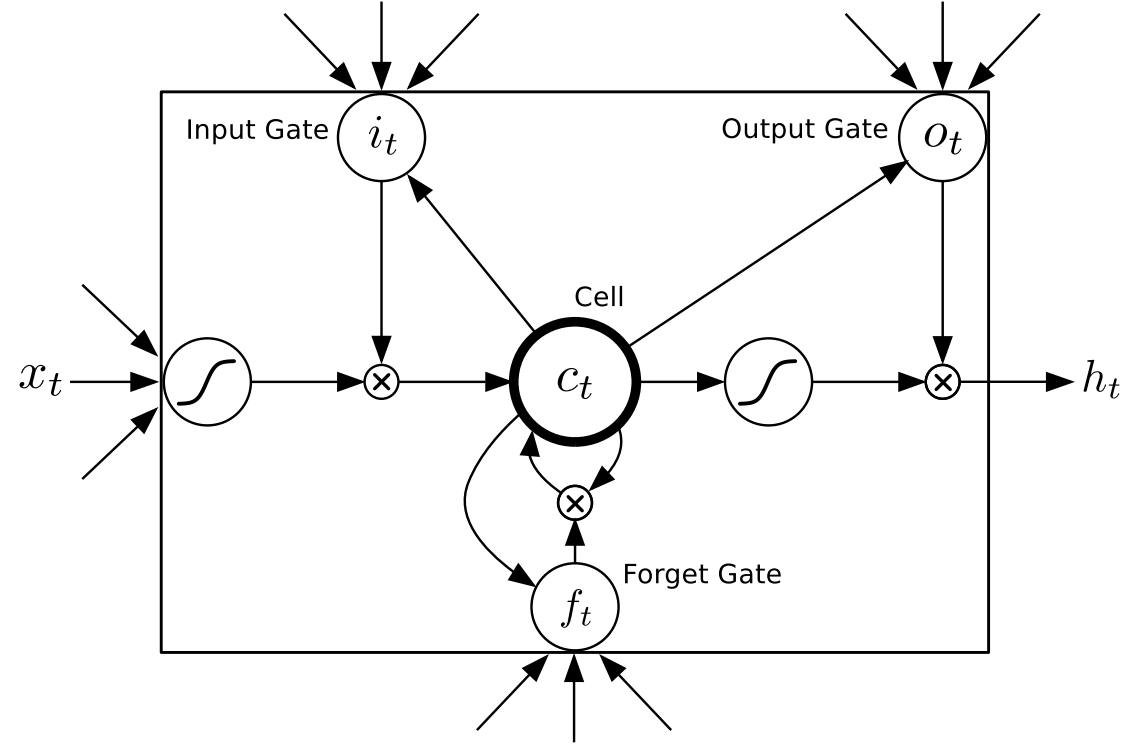
\includegraphics[width=\linewidth]{LSTM}
  \caption{An LSTM Module}
  \label{fig:LSTM}
\end{figure}


Using LSTMs in modeling source code is arguable more important than in the natural language modeling case. It has been shown that although computationally expensive, modest sized $n-gram$ models can model languages well, and can predict the next word well. However, this is due to the fact that natural language is fairly local. Most words (or characters) do not heavily depend on words farther than about 20 back. In the source code case, it is drastically different. For example, a function could be 20 lines (and thus $>$ about 200 tokens) long. The characters at the end of the function are heavily dependent on the characters at the beginning of the function, and possibly even lines before the function. Recently, it was shown by \cite{karpathy2015visualizing} that we can easily generate source code which appears to be written by a human, from a source code language model. This is most impressive because in the examples shown, the code is well indented, the braces and brackets are correctly nested, and even commented correctly. This is not something that can be achieved by looking at the previous $n$ characters.

\subsection{Experimental Setup}


\section{Results}


\section{Threats to Validity}

\section{Conclusion}



% In the unusual situation where you want a paper to appear in the
% references without citing it in the main text, use \nocite


\bibliography{example_paper}
\bibliographystyle{icml2015}

\end{document} 


% This document was modified from the file originally made available by
% Pat Langley and Andrea Danyluk for ICML-2K. This version was
% created by Lise Getoor and Tobias Scheffer, it was slightly modified  
% from the 2010 version by Thorsten Joachims & Johannes Fuernkranz, 
% slightly modified from the 2009 version by Kiri Wagstaff and 
% Sam Roweis's 2008 version, which is slightly modified from 
% Prasad Tadepalli's 2007 version which is a lightly 
% changed version of the previous year's version by Andrew Moore, 
% which was in turn edited from those of Kristian Kersting and 
% Codrina Lauth. Alex Smola contributed to the algorithmic style files.  
